\documentclass{beamer}
\usetheme{Boadilla}
\beamertemplatenavigationsymbolsempty

\title{Dungeons and Bindings}
\subtitle{Entwicklungsprozess}
\author{Frederik, Leandro}
\institute{TU Dortmund}

\date{14. Juli 2020}

\begin{document}

\begin{frame}
\titlepage
\end{frame}

\begin{frame}{Inhalt}
\tableofcontents
\end{frame}

\section{Zielsetzung}
%\begin{frame}{Zielsetzung}
\begin{itemize}
\item Dungeon Crawl
\begin{itemize}
    \item Navigation durch Dungeon mit Gegnern, Gegenständen etc.
    \item Bewältigung des Dungeons durch Powerups
\end{itemize}
\item Rogue-like
\begin{itemize}
    \item prozedural generierte Level und rundenbasierte Spielweise
    \item eine Runde: Level erfolgreich/erfolglos beenden (Sieg/ Game Over)
\end{itemize}
\end{itemize}
\end{frame}

\begin{frame}{Problemstellung}
\begin{itemize}
    \item Dungeongenerierung: Welches PCG-Verfahren? 
    \begin{itemize}
        \item L-Systems
    \end{itemize}
    \item Raumlayouts innerhalb von Dungeon (Hindernisse etc.) ?
    \begin{itemize}
        \item Variabilität
    \end{itemize}
    \item Größe Itempool/Gegnerpool?
    \begin{itemize}
        \item Großer Bestandteil des Spiels
    \end{itemize}
    \item Typen von Items/Gegnern: Welches KI-Verfahren?
    \begin{itemize}
        \item Steering Behaviors
    \end{itemize}
\end{itemize}
\end{frame}

\section{Schwerpunkte}

\subsection{L-Systems}
%\begin{frame}
\vfill
\centering
\begin{beamercolorbox}[sep=8pt,center,shadow=true,rounded=true]{title}
\usebeamerfont{title}L-Systems
\end{beamercolorbox}
\vfill
\end{frame}

\begin{frame}
\frametitle{Anforderungen an die Dungeongenerierung}

\begin{itemize}
\item Ebenen generieren mit n Räumen
\item Genau ein Boss- und ein Loot-Raum
\item Alle Räume sind gleich groß und rechteckig
\item Benachbarte Räume können, müssen aber nicht verbunden sein
\item Kreise sollen möglich sein
\item Jeder Raum muss vom Startraum aus erreichbar sein
\end{itemize}

\end{frame}

\begin{frame}
\frametitle{L-Systems (Lindenmayer Systems)}

\begin{itemize}
\item Raumstrukturen werden über Grammatiken erzeugt
\item Alphabet: S, L, B, 1, 2, 3, 4
\item Startsymbol: S
\item Ersetzungsregeln zweidimensional
\end{itemize}

\end{frame}

\begin{frame}
\frametitle{Regeln}

\begin{itemize}
\item Anfügeregeln: z.B.: S: S-3, 2: 2-4 2: 2-L
\item Verschiebunsgregeln: z.B.: B: 2-B, L: 3-L
\item Sonderzwangsregeln: z.B.: 2: 3-B, 3: 4-L
\item Räume können nur erzeugt werden, wenn dort noch kein Raum ist und wenn die zulässige Türenanzahl nicht überschritten wird (1 bei L und B, 4 bei S)
\item Genau n-2 nicht L oder B Räume
\item Regeln werden inaktiv, wenn Randbedingungen nicht gelten
\item Generierte Räume verbinden sich wenn erlaubt mit benachbarten Räumen
\item Regeln haben Gewichte um die Ebenen interessanter zu machen
\end{itemize}

\end{frame}

\begin{frame}
\frametitle{Generierungsprozess}

\begin{itemize}
\item Wähle zufällig einen bestehenden Raum aus
\item Prüfe welche Regeln darauf anwendbar sind
\item Wende eine zufällige dieser Regeln an, wiederhole das ganze
\item Anderen Raum auswählen wenn keine Regel anwendbar ist
\item Abbruch wenn kein Raum anwendbare Regeln besitzt
\item Wähle für jeden Raum ein zufälliges Raum-Preset für diesen Raumtyp
\item Erstelle die Räume als entsprechende Spielszenen
\end{itemize}

\end{frame}

\begin{frame}
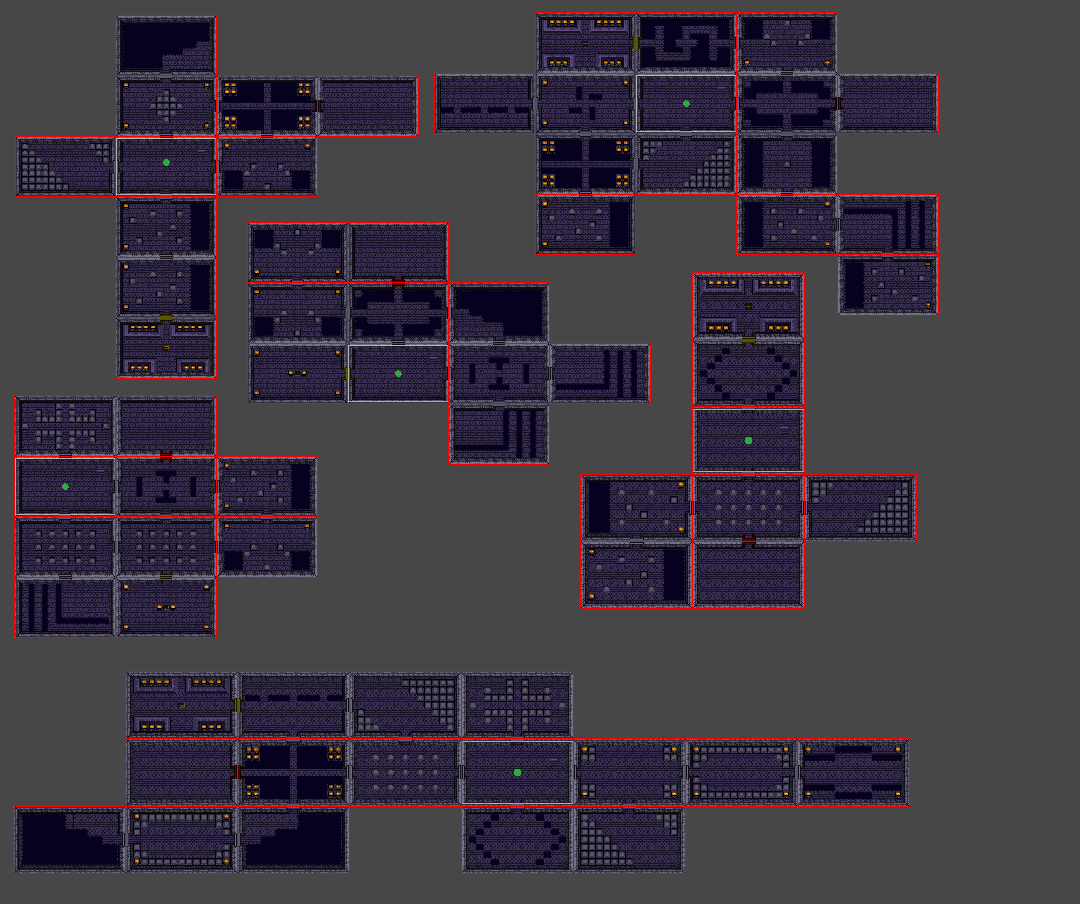
\includegraphics[scale=0.39]{Bilder/EbenenCollage}
\end{frame}



\subsection{Steering-Behaviors}
%\begin{frame}
\vfill
\centering
\begin{beamercolorbox}[sep=8pt,center,shadow=true,rounded=true]{title}
\usebeamerfont{title}Steering Behaviors
\end{beamercolorbox}
\vfill
\end{frame}

\begin{frame}{Anforderungen an Gegner}
\begin{itemize}
    \item Gegner sollen unterschiedliches Verhalten zeigen können (Fliehend, Zielsuchend, Wandernd etc.)
    \item Verhalten soll änderbar sein (z.B. durch Items)
    \newline
    \setbeamertemplate{itemize item}[triangle]
    \item Steering Behaviors
\end{itemize}
\end{frame}

\section{Gameplay-Elemente}
%\include{Kapitel/Gameplay-Elemente}

\section{Fazit}
%\include{Kapitel/Fazit}

\end{document}